\documentclass[10pt, a4paper, oneside]{article}
\usepackage[hidelinks]{hyperref}
\usepackage{jucs2e}
\usepackage{graphicx}
\usepackage{url}
\usepackage{mathtools}
\usepackage{scalerel}
\usepackage{setspace}
\usepackage[strict]{changepage}
\usepackage[letterspace=-50]{microtype}
\usepackage{fontspec}
\usepackage{afterpage}
\usepackage{ragged2e}
\usepackage{booktabs}
\usepackage{listings}
\usepackage{xcolor}
\usepackage{array}
\usepackage{tabularx}

\setmainfont{Times New Roman}

\usepackage{titlesec}
\titleformat*{\section}{\Large\bfseries}
\titleformat*{\subsection}{\normalsize\bfseries}

\renewcommand{\baselinestretch}{0.9}

\graphicspath{{./figures/}}

\usepackage[textwidth=8cm, margin=0cm, left=4.6cm, right=4.2cm, top=3.9cm, bottom=6.8cm, a4paper, headheight=0.5cm, headsep=0.5cm]{geometry}
\usepackage{fancyhdr}
\usepackage[format=plain, labelfont=it, textfont=it, justification=centering]{caption}
\usepackage{breakcites}

\apptocmd{\frame}{}{\justifying}{}

\urlstyle{same}
\pagestyle{fancy}

%% TypeScript code listing style
\lstdefinestyle{typescript}{
  language=Java,
  basicstyle=\small\ttfamily,
  keywordstyle=\color{blue}\bfseries,
  commentstyle=\color{green!60!black}\itshape,
  stringstyle=\color{red!70!black},
  numbers=left,
  numberstyle=\tiny\color{gray},
  numbersep=5pt,
  frame=single,
  breaklines=true,
  captionpos=b,
  showstringspaces=false,
  tabsize=2,
  columns=flexible,
  morekeywords={async,await,const,let,import,export,from,interface,type,extends,implements,readonly,Promise,string,number,boolean,void,undefined,null,true,false,new,throw,try,catch,finally},
  deletekeywords={super}
}

\newcommand\jucs{{Journal of Universal Computer Science}}
\newcommand\jucsvol{vol. XX, no. X (2026)}
\newcommand\jucspages{1-25}
\newcommand\jucssubmitted{XX/XX/2026}
\newcommand\jucsaccepted{XX/XX/2026}
\newcommand\jucsappeared{XX/XX/2026}
\newcommand\jucslicence{ CC BY 4.0}
\newcommand\startingPage{1}
\setcounter{page}{\startingPage}

\newcommand\paperauthor{{Al Ghanimi, A.: }}
\newcommand\papertitle{IraqPay: A Unified Open-Source Payment SDK for Fragmented Gateway Ecosystems in Emerging Markets}

\header{\paperauthor \papertitle}

\begin{document}

\title{{\fontsize{14pt}{14pt}\selectfont{\vspace*{-3mm}\papertitle\vspace*{-1mm}}}}

\author{{\bfseries\fontsize{10pt}{10pt}\selectfont{Ali Al~Ghanimi}} \\
   {\fontsize{9pt}{12pt}\selectfont{(Department of Electrical Engineering, Faculty of Engineering,\\University of Kufa, Najaf, Iraq\\
   \orcid{0000-0000-0000-0000},
   ali.alghanimi@uokufa.edu.iq)}}
}

\label{first}
\maketitle

{\fontfamily{ptm}\selectfont
\begin{abstract}
{\fontsize{9pt}{9pt}\selectfont{\vspace*{-2mm}
Payment infrastructure in emerging markets is often fragmented across multiple incompatible gateways, each with distinct authentication protocols, API conventions, and operational constraints. This paper presents IraqPay, the first open-source unified SDK that integrates five Iraqi payment gateways---ZainCash, First Iraqi Bank (FIB), QiCard, NassPay, and Cash-on-Delivery---through a single TypeScript API. Beyond gateway unification, IraqPay provides production-grade infrastructure: a circuit breaker for fault tolerance, a smart router with three routing strategies and automatic fallback chains, per-gateway analytics with latency percentiles and error breakdowns, request tracing with correlation IDs, and a benchmark suite for systematic performance comparison. We present the software architecture based on the adapter design pattern, analyze the heterogeneous authentication landscape, and provide benchmark results from live sandbox testing. IraqPay is deployed in a production food marketplace, published on npm, and available under the MIT license at \url{https://github.com/Balghanimi/iraqpay}.}}
\end{abstract}}

{\fontfamily{ptm}\selectfont
\begin{keywords}
{\fontsize{9pt}{9pt}\selectfont{
payment gateway, unified SDK, emerging markets, Iraq, fintech, open source, adapter pattern, circuit breaker}}
\end{keywords}}

{\fontfamily{ptm}\selectfont
\begin{category}
{\fontsize{9pt}{9pt}\selectfont{
D.2.11 [Software Architectures]: Patterns, D.2.13 [Reusable Software]: Reusable libraries, H.3.5 [Online Information Services]: Web-based services, J.1 [Administrative Data Processing]: Financial}}
\end{category}}

{\fontfamily{ptm}\selectfont
\begin{doi}
{\fontsize{9pt}{9pt}\selectfont{
10.3897/jucs.\textless SubmissionNumber\textgreater}}
\end{doi}}


\section{Introduction}

Digital payment adoption in Iraq has accelerated rapidly since 2020, driven by mobile money services, government salary digitization, and post-pandemic e-commerce growth~[GSMA (2023)]. However, unlike mature markets where a single aggregator (e.g., Stripe, Adyen) provides a unified interface~[Stripe (2023)], the Iraqi payment landscape remains \emph{fragmented}: developers must integrate each gateway individually, dealing with five fundamentally different APIs, authentication schemes, response formats, and operational constraints.

This fragmentation creates several problems. First, each gateway requires bespoke code for authentication, request construction, response parsing, and callback verification---multiplied by the number of gateways supported. Second, error codes, formats, and recovery strategies differ across gateways, making unified error handling difficult. Third, if a gateway experiences downtime, applications have no mechanism to automatically route payments to an alternative. Fourth, developers lack built-in tools to compare gateway performance or diagnose failures.

Global payment aggregators (Stripe, PayPal, Adyen) do not operate in Iraq. Regional aggregators such as HyperPay and PayTabs serve parts of the Middle East but have limited or no Iraqi gateway coverage. To our knowledge, no open-source SDK provides unified access to Iraqi payment gateways.

This paper presents IraqPay, a unified open-source TypeScript SDK that addresses this gap by providing: (1)~a unified adapter-pattern SDK abstracting five Iraqi gateways behind a single API, (2)~production infrastructure including a circuit breaker, smart router, analytics engine, and request tracer, and (3)~a benchmark suite for systematic gateway performance comparison. The approach generalizes to any fragmented payment ecosystem in emerging markets.

The remainder of this paper is organized as follows. Section~2 presents related work. Section~3 describes the software architecture. Section~4 provides illustrative usage examples. Section~5 presents benchmark results. Section~6 discusses a production case study. Section~7 analyzes generalizability and impact. Section~8 concludes.


\section{Related Work}

\subsection{Payment Aggregation}

Payment aggregation SDKs consolidate multiple payment providers behind a unified interface. Stripe~[Stripe (2023)] is the dominant example in Western markets, supporting hundreds of payment methods across dozens of countries. However, Stripe does not operate in Iraq or most of the Middle East. Similar limitations apply to Adyen, Braintree, and Square.

Regional aggregators have emerged to serve underserved markets. Paystack~[Paystack (2024)] serves West Africa (primarily Nigeria and Ghana), while Razorpay~[Razorpay (2024)] dominates the Indian market. HyperPay and PayTabs operate in parts of the Middle East but provide limited or no coverage for Iraqi gateways such as ZainCash and QiCard.

\subsection{Fault Tolerance in Payment Systems}

The circuit breaker pattern, first described by Nygard~[Nygard (2018)] and popularized by Fowler~[Fowler (2014)], is widely used in microservice architectures to prevent cascading failures. Netflix's Hystrix library was among the first production implementations. In payment systems, circuit breakers are particularly important because gateway outages should not prevent all payments---they should trigger failover to alternative gateways.

\subsection{Software Design Patterns}

The adapter pattern~[Gamma et al. (1994)] provides the architectural foundation for IraqPay. By defining a common interface (\texttt{PaymentGateway}) and implementing gateway-specific adapters, the system decouples application logic from gateway-specific details. This pattern is well-established in software engineering but, to our knowledge, has not been applied to Iraqi payment gateway unification in an open-source context.


\section{Software Architecture}

\subsection{Overview}

IraqPay employs the adapter pattern to abstract gateway heterogeneity behind a uniform interface. Figure~\ref{fig:architecture} illustrates the overall architecture. The core abstraction is the \texttt{PaymentGateway} interface:

\begin{lstlisting}[style=typescript,caption={Core gateway interface},label={lst:interface}]
interface PaymentGateway {
  readonly name: GatewayName;
  createPayment(params): Promise<PaymentResult>;
  getStatus(paymentId: string): Promise<PaymentStatusResult>;
  cancel(paymentId: string, amount?: number): Promise<boolean>;
  refund(paymentId: string, amount?: number): Promise<boolean>;
  verifyCallback(payload: unknown): Promise<WebhookEvent>;
}
\end{lstlisting}

Each gateway adapter encapsulates its specific authentication protocol, API endpoint construction, request/response mapping, and callback verification logic. The \texttt{IraqPay} orchestrator manages gateway lifecycle and delegates operations through three infrastructure layers: (1)~a smart router for gateway selection, (2)~a circuit breaker for fault tolerance, and (3)~an analytics and tracing engine for observability.

\begin{figure}[h]
    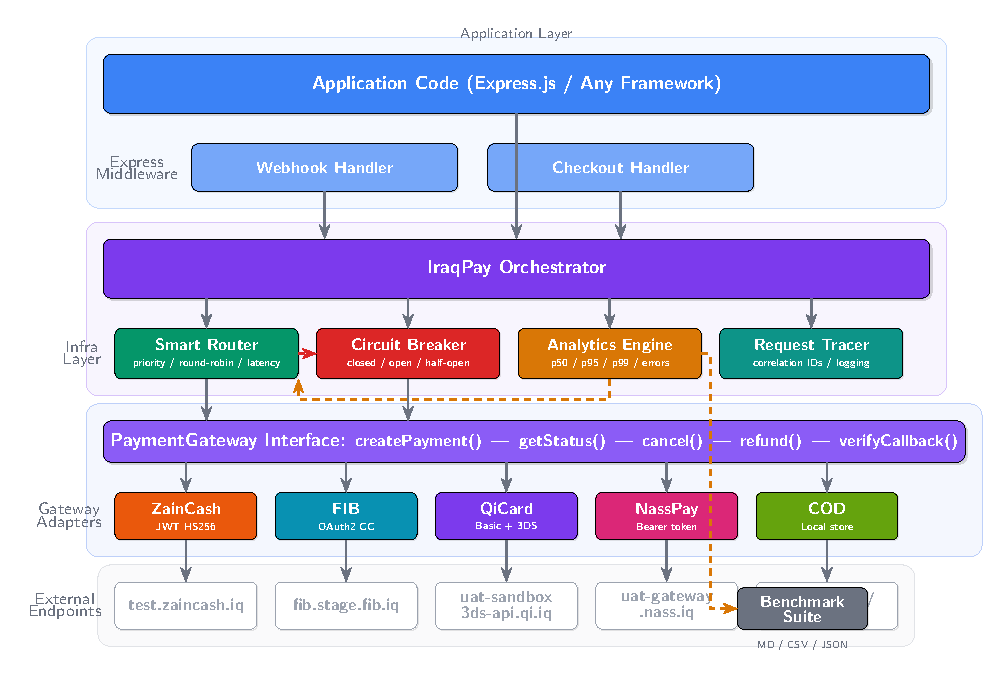
\includegraphics[width=\textwidth]{architecture.pdf}
    \centering
    \captionsetup{font=small}
    \caption{\fontsize{10pt}{11pt}\selectfont{\itshape{IraqPay architecture. The orchestrator delegates payment operations through the smart router and circuit breaker to gateway adapters, while the analytics engine and tracer record all operations.}}}
    \label{fig:architecture}
\end{figure}

\subsection{Gateway Heterogeneity}

Table~\ref{table:gateway-comparison} summarizes the heterogeneity across the five Iraqi gateways. Each implements a fundamentally different authentication mechanism.

\begin{table}[ht]
    \centering
    \setlength\tabcolsep{3pt}
    \small
    \begin{tabular}{llllll}
        \toprule
        \bfseries Feature & \bfseries ZainCash & \bfseries FIB & \bfseries QiCard & \bfseries NassPay & \bfseries COD \\
        \midrule
        Auth & JWT HS256 & OAuth2 CC & Basic+Header & Bearer & None \\
        Flow & Redirect & QR+deep links & 3DS redirect & 3DS redirect & Internal \\
        Currencies & IQD & IQD, USD & IQD & IQD, USD & Any \\
        API refund & No & Yes & Yes & No & Manual \\
        API cancel & No & Yes & Yes & No & Internal \\
        Webhooks & JWT callback & POST JSON & POST & POST & --- \\
        Min. amount & 250 IQD & --- & --- & --- & --- \\
        Status window & Unlimited & Unlimited & Unlimited & 24 hours & Unlimited \\
        \bottomrule
    \end{tabular}
    \caption{\fontsize{10pt}{11pt}\selectfont{\itshape{Comparison of Iraqi payment gateway characteristics.}}}
    \label{table:gateway-comparison}
\end{table}

\textbf{ZainCash} uses JWT (HS256) for both request signing and callback verification. Payment parameters are encoded in a signed JWT and submitted to the API, which returns a transaction ID and redirect URL.

\textbf{FIB (First Iraqi Bank)} implements OAuth2 client credentials flow with automatic token refresh. Successful payment creation returns a QR code (base64), a human-readable code, and three mobile deep links. The SDK handles 401 responses by transparently re-authenticating and retrying.

\textbf{QiCard} uses HTTP Basic authentication with an additional \texttt{X-Terminal-Id} header. The SDK always performs server-side status verification on callback receipt---a security best practice preventing client-side tampering.

\textbf{NassPay} authenticates via a login endpoint returning a Bearer token with a time-to-live. The SDK implements conservative token caching with a 50-minute TTL and automatic retry on 401 responses.

\textbf{COD (Cash-on-Delivery)} is a local state tracker with a pluggable storage interface, allowing developers to substitute in-memory storage with a database adapter.

\subsection{Circuit Breaker}

The circuit breaker implements the standard three-state pattern~[Nygard (2018), Fowler (2014)] with per-gateway isolation:

\begin{itemize}
\item \textbf{Closed} (normal): Requests pass through. Consecutive failures are counted.
\item \textbf{Open} (failing): Requests are immediately rejected. After a configurable reset timeout (default: 30s), the circuit transitions to half-open.
\item \textbf{Half-open} (testing): A limited number of test requests are allowed. If they succeed, the circuit closes; if any fail, it reopens.
\end{itemize}

Configuration supports per-gateway overrides, allowing different failure thresholds for gateways with known reliability differences.

\subsection{Smart Router}

The smart router supports three strategies:

\textbf{Priority:} Each gateway is assigned a numerical priority; the lowest value is selected first.

\textbf{Round-robin:} Gateways are cycled in order, distributing load evenly. Useful for A/B testing.

\textbf{Lowest-latency:} The gateway with the lowest median (p50) latency from the analytics engine is selected, adapting dynamically to performance changes.

All strategies respect gateway rules (minimum/maximum amounts, supported currencies) and circuit breaker state. When the primary gateway fails, the router provides a fallback chain of alternatives.

\subsection{Analytics and Tracing}

The analytics engine collects metrics in a sliding window (configurable, default 1000 samples per gateway) and exposes per-gateway latency percentiles (p50, p95, p99), success/failure rates, error breakdowns by code, and real-time event listeners.

The tracing module assigns unique 128-bit correlation IDs to every payment operation. A structured \texttt{Logger} interface allows integration with any logging framework. Log entries include trace ID, span ID, gateway name, operation type, duration, and optional metadata.

\subsection{Benchmark Suite}

The benchmark runner executes $N$ payment iterations per gateway and produces structured reports with per-gateway latency statistics (min, max, average, median, p95, p99, standard deviation), success rates, error distributions, and comparison tables. Reports can be exported to Markdown, CSV, and JSON formats.


\section{Illustrative Examples}

\subsection{Basic Usage}

\begin{lstlisting}[style=typescript,caption={Basic payment creation with two gateways},label={lst:basic}]
import { IraqPay } from 'iraqpay';

const pay = new IraqPay({
  gateways: {
    zaincash: { msisdn: '...', merchantId: '...', secret: '...' },
    fib: { clientId: '...', clientSecret: '...' },
  },
  sandbox: true,
});

const payment = await pay.createPayment({
  gateway: 'zaincash',
  amount: 25000,
  orderId: 'order_123',
  callbackUrl: 'https://myapp.com/callback',
});
console.log(payment.redirectUrl); // Redirect user here
\end{lstlisting}

\subsection{Smart Routing with Fallback}

\begin{lstlisting}[style=typescript,caption={Automatic gateway selection with fallback},label={lst:routing}]
const pay = new IraqPay({
  gateways: { zaincash: {...}, fib: {...}, qicard: {...} },
  router: {
    enabled: true,
    strategy: 'lowest-latency',
    fallbackChain: ['fib', 'zaincash', 'qicard'],
    rules: {
      zaincash: { minAmount: 250, currencies: ['IQD'] },
      fib: { currencies: ['IQD', 'USD'] },
    },
  },
  circuitBreaker: { failureThreshold: 3 },
  analytics: { enabled: true },
});

// No gateway specified -- router selects automatically
const payment = await pay.createPayment({
  amount: 10000, orderId: 'order_456',
  callbackUrl: 'https://myapp.com/webhook',
});
\end{lstlisting}

\subsection{Production Monitoring}

\begin{lstlisting}[style=typescript,caption={Accessing per-gateway metrics and events},label={lst:metrics}]
const metrics = pay.analytics.getMetrics();
for (const [gw, m] of Object.entries(metrics.byGateway)) {
  console.log(`${gw}: ${(m.successRate*100).toFixed(1)}% success, `
    + `p50=${m.p50Ms}ms, p95=${m.p95Ms}ms`);
}

// Real-time failure alerting
pay.analytics.on((event) => {
  if (!event.success)
    alertOps(`${event.gateway} failed: ${event.error?.message}`);
});
\end{lstlisting}


\section{Benchmark Results}

To characterize gateway performance, we executed 50 payment creation requests against the ZainCash sandbox and COD gateway, and 10 network reachability probes against FIB, QiCard, and NassPay sandbox endpoints. All benchmarks were executed from Najaf, Iraq. Table~\ref{table:benchmarks} summarizes the results.

\begin{table}[ht]
    \centering
    \setlength\tabcolsep{4pt}
    \small
    \begin{tabular}{lrrrrrrr}
        \toprule
        \bfseries Gateway & \bfseries N & \bfseries Success & \bfseries Avg & \bfseries Med & \bfseries P95 & \bfseries P99 & \bfseries StdDev \\
        & & \bfseries (\%) & \bfseries (ms) & \bfseries (ms) & \bfseries (ms) & \bfseries (ms) & \bfseries (ms) \\
        \midrule
        ZainCash & 50 & 100 & 279 & 248 & 391 & 934 & 113 \\
        COD & 50 & 100 & $<$1 & $<$1 & $<$1 & $<$1 & $<$1 \\
        \midrule
        \multicolumn{8}{l}{\itshape Network reachability probes (auth fails, measures endpoint RTT):} \\
        FIB$^\dagger$ & 10 & 0 & 137 & 188 & --- & --- & --- \\
        QiCard$^\dagger$ & 10 & 0 & 150 & 171 & --- & --- & --- \\
        NassPay$^\dagger$ & 10 & 0 & 127 & 167 & --- & --- & --- \\
        \bottomrule
    \end{tabular}
    \caption{\fontsize{10pt}{11pt}\selectfont{\itshape{Gateway benchmark results (sandbox mode, March 2026). $^\dagger$FIB, QiCard, and NassPay require merchant registration for valid sandbox credentials; probe latencies reflect network RTT to first HTTP error response.}}}
    \label{table:benchmarks}
\end{table}

ZainCash exhibits stable performance with a median latency of 248~ms and 100\% success rate over 50 consecutive requests. The first request shows a cold-start penalty (934~ms), after which latency stabilizes in the 229--355~ms range. The COD gateway, being purely local, operates at sub-millisecond latency. Network probes to FIB, QiCard, and NassPay confirm that all sandbox endpoints are reachable from Iraq with round-trip times of 127--188~ms, consistent with regional hosting.


\section{Case Study: Akel Bait Food Marketplace}

IraqPay is deployed in \emph{Akel Bait}, a production food marketplace serving customers in Iraqi cities. The application uses IraqPay to offer ZainCash mobile payments alongside cash-on-delivery, with the smart router configured to fall back to COD when ZainCash is unavailable.

The integration required fewer than 20 lines of application code---a single \texttt{IraqPay} instantiation and a \texttt{createPayment} call in the checkout flow. The Express.js webhook middleware handles all callback verification and status updates automatically. The analytics engine provides the operations team with real-time visibility into payment success rates and gateway latency, enabling data-driven decisions about which gateways to prioritize.


\section{Impact and Generalizability}

While IraqPay targets the Iraqi market, its architecture is intentionally general. The adapter pattern, circuit breaker, smart router, and analytics engine are gateway-agnostic---adding a new gateway requires only implementing the \texttt{PaymentGateway} interface (five methods). This makes the pattern directly applicable to other fragmented payment ecosystems, such as Bangladesh (bKash, Nagad, Rocket, SSLCommerz), Pakistan (JazzCash, EasyPaisa, HBL), Nigeria (Paystack, Flutterwave, Interswitch), and Egypt (Fawry, Paymob, Accept).

The open-source availability (MIT license) and npm distribution model lower the barrier for developers in these markets to either adopt IraqPay directly or fork it as a starting point. The benchmark suite provides a methodological contribution: a standardized, reproducible approach to comparing payment gateway performance that is currently absent from the fintech ecosystem.

\subsection{AI Tool Disclosure}

In accordance with J.UCS policy, we disclose that Claude (Anthropic, Claude Opus 4.6) was used as a coding assistant during the development of IraqPay's source code and during manuscript preparation. All code was reviewed, tested, and validated by the author. The author retains full responsibility for the correctness and originality of all content.


\section{Conclusions and Future Work}

IraqPay demonstrates that payment gateway fragmentation in emerging markets can be effectively addressed through a well-designed adapter-pattern SDK with production-grade infrastructure. The key contributions are:

\begin{enumerate}
\item The first open-source unified SDK for Iraqi payment gateways, abstracting five heterogeneous APIs behind a single interface.
\item Production infrastructure (circuit breaker, smart router, analytics, tracing) that goes beyond simple API unification to address real-world reliability and observability requirements.
\item A benchmark suite enabling systematic, reproducible gateway performance comparison.
\item An architecture pattern that generalizes to any fragmented payment ecosystem.
\end{enumerate}

The software is published on npm (\texttt{npm install iraqpay}), available on GitHub under the MIT license, and deployed in a production food marketplace. The codebase comprises approximately 5,000 lines of TypeScript with 111 passing tests across 13 test suites.

Future work includes adding support for subscription and recurring payments, integrating additional Middle Eastern gateways (e.g., Iraqi mobile wallets), conducting a longitudinal production reliability study, and investigating machine-learning-based gateway selection that adapts to time-of-day and transaction-type patterns.

\begin{Acknowledgements}
This work was supported by the University of Kufa, Faculty of Engineering.
\end{Acknowledgements}


\begin{thebibliography}{}{
\fontsize{9pt}{10pt}\selectfont

\bibitem[Fowler (2014)]{fowler2014} Fowler, M.: ``Circuit Breaker''; \url{https://martinfowler.com/bliki/CircuitBreaker.html} (2014).

\bibitem[Gamma et~al. (1994)]{gamma1994} Gamma, E., Helm, R., Johnson, R., Vlissides, J.: ``Design Patterns: Elements of Reusable Object-Oriented Software''; Addison-Wesley (1994).

\bibitem[GSMA (2023)]{gsma2023} GSMA: ``State of the Industry Report on Mobile Money 2023''; GSMA, London (2023).

\bibitem[Nygard (2018)]{nygard2018} Nygard, M.~T.: ``Release It!: Design and Deploy Production-Ready Software''; Pragmatic Bookshelf, 2nd edition (2018).

\bibitem[Paystack (2024)]{paystack2024} Paystack: ``Paystack Developer Documentation''; \url{https://paystack.com/docs} (2024).

\bibitem[Razorpay (2024)]{razorpay2024} Razorpay: ``Razorpay API Reference''; \url{https://razorpay.com/docs/api} (2024).

\bibitem[Stripe (2023)]{stripe2023} Stripe, Inc.: ``Stripe API Reference''; \url{https://stripe.com/docs/api} (2023).

\bibitem[World Bank (2023)]{worldbank2023} World Bank: ``Iraq Economic Monitor: Navigating Uncertainty''; World Bank Group, Washington, D.C. (2023).

\bibitem[ZainCash (2024)]{zaincash2024} Zain Cash: ``ZainCash API Documentation''; \url{https://docs.zaincash.iq} (2024).

\bibitem[FIB (2024)]{fib2024} First Iraqi Bank: ``FIB Payment Gateway Developer Guide''; \url{https://fib.iq} (2024).

}\end{thebibliography}

\end{document}
